\chapter{Microkernel/Plugin Architecture}

\section{Pendahuluan}

Dalam dunia komputasi modern, kebutuhan akan sistem yang modular, fleksibel, dan dapat diperluas semakin meningkat. Arsitektur perangkat lunak memainkan peran penting dalam menentukan bagaimana sistem dapat berkembang dan beradaptasi terhadap perubahan. Dua pendekatan utama yang sering digunakan untuk mencapai modularitas dan fleksibilitas adalah \textbf{microkernel} dan \textbf{plugin architecture}.

Arsitektur \textbf{microkernel} muncul sebagai solusi terhadap keterbatasan sistem operasi monolitik yang memiliki ketergantungan tinggi antar komponen dan sulit untuk diperbarui. Dengan pendekatan ini, hanya fungsi-fungsi inti yang berjalan di dalam kernel, sedangkan layanan tambahan seperti sistem file, driver perangkat, dan manajemen jaringan ditempatkan sebagai proses terpisah di ruang pengguna. Desain ini memberikan keuntungan dalam hal keamanan dan stabilitas karena kegagalan pada satu layanan tidak akan mempengaruhi keseluruhan sistem.

Di sisi lain, \textbf{plugin architecture} berkembang sebagai cara untuk menambahkan fitur secara dinamis dalam suatu perangkat lunak tanpa harus mengubah kode inti. Pendekatan ini memungkinkan pengembang untuk menambahkan atau mengganti fungsionalitas tanpa perlu melakukan rekonstruksi sistem utama. Banyak aplikasi modern seperti Integrated Development Environment (IDE), sistem manajemen konten (CMS), dan perangkat lunak multimedia mengadopsi arsitektur berbasis plugin untuk meningkatkan fleksibilitas dan kemudahan ekspansi.

Pada dokumen ini, akan dibahas konsep dan penerapan arsitektur \textbf{microkernel} serta \textbf{plugin}, termasuk sejarah perkembangan, contoh implementasi, keunggulan dan kelemahan, serta cara penerapan dalam proyek perangkat lunak berbasis Java. Dengan memahami kedua arsitektur ini, pengembang dapat memilih pendekatan yang sesuai dengan kebutuhan sistem yang sedang dibangun.

\section{Sejarah dan Perkembangan}

Konsep \textbf{microkernel} muncul sebagai respons terhadap keterbatasan arsitektur sistem operasi monolitik. Pada awalnya, sistem operasi dirancang menggunakan pendekatan monolitik di mana semua layanan sistem, termasuk manajemen memori, sistem file, dan driver perangkat keras, terintegrasi dalam satu unit kernel yang besar. Pendekatan ini memberikan performa yang baik tetapi memiliki beberapa kelemahan, seperti kurangnya fleksibilitas, kesulitan dalam pemeliharaan, serta kerentanan terhadap kesalahan sistem yang menyebabkan kegagalan total (\textit{system crash}).

Pada tahun 1960-an dan 1970-an, penelitian dalam desain sistem operasi mulai mengeksplorasi pendekatan modular untuk meningkatkan keandalan dan keamanan. Salah satu sistem awal yang mengadopsi prinsip microkernel adalah \textbf{THE Operating System}, yang dikembangkan oleh Edsger W. Dijkstra pada tahun 1968. Meskipun belum sepenuhnya menerapkan konsep microkernel, sistem ini memperkenalkan gagasan pembagian sistem operasi menjadi beberapa lapisan dengan fungsi yang terpisah.

Pada tahun 1980-an, arsitektur microkernel mulai mendapatkan perhatian yang lebih besar. Salah satu proyek paling berpengaruh adalah \textbf{Mach}, yang dikembangkan di Carnegie Mellon University. Mach memperkenalkan konsep bahwa hanya fungsi inti seperti manajemen memori, penjadwalan proses, dan komunikasi antarproses (\textit{Inter-Process Communication} atau IPC) yang dijalankan dalam kernel, sementara layanan lain seperti sistem file dan driver perangkat keras ditempatkan dalam proses pengguna. Pendekatan ini meningkatkan modularitas dan keamanan, tetapi sering kali mengalami penurunan performa karena overhead komunikasi antarproses.

Pada tahun 1990-an, microkernel terus berkembang dengan munculnya sistem seperti \textbf{L4}, yang dirancang untuk mengatasi keterbatasan performa dari microkernel generasi sebelumnya. L4 menekankan efisiensi dalam mekanisme komunikasi antarproses dan memberikan fondasi bagi berbagai implementasi modern, termasuk QNX dan Minix.

Di sisi lain, konsep \textbf{plugin architecture} mulai berkembang dalam dunia perangkat lunak sebagai cara untuk memperkenalkan modularitas pada aplikasi. Awalnya, sistem perangkat lunak dibangun sebagai monolitik, di mana semua fitur dikompilasi ke dalam satu kode sumber utama. Namun, dengan meningkatnya kompleksitas perangkat lunak, pendekatan ini menjadi sulit untuk dikelola dan diperbarui.

Pada tahun 1990-an, perangkat lunak seperti \textbf{Netscape Navigator} dan \textbf{Microsoft Internet Explorer} mulai mengadopsi arsitektur berbasis plugin, memungkinkan pengembang pihak ketiga untuk menambahkan fitur baru ke dalam aplikasi tanpa perlu memodifikasi kode inti. Konsep ini kemudian diperluas ke berbagai jenis perangkat lunak, termasuk sistem manajemen konten (\textbf{CMS}), Integrated Development Environment (\textbf{IDE}) seperti Eclipse dan Visual Studio, serta platform game seperti Unreal Engine.

Saat ini, baik microkernel maupun plugin architecture digunakan secara luas dalam berbagai sistem, termasuk sistem operasi real-time, embedded systems, hypervisor virtualisasi, serta aplikasi skala besar yang memerlukan fleksibilitas tinggi dan modularitas yang kuat.


\section{Penerapan dalam Dunia Nyata}

Arsitektur \textbf{microkernel} dan \textbf{plugin} memiliki berbagai penerapan dalam dunia nyata, terutama dalam bidang sistem operasi, aplikasi perangkat lunak, dan sistem tertanam (\textit{embedded systems}). Penerapan ini menunjukkan keunggulan desain modular, fleksibilitas, serta peningkatan keamanan dan stabilitas dalam pengelolaan sistem yang kompleks.

\subsection{Penerapan Microkernel dalam Sistem Operasi}

Microkernel digunakan dalam berbagai sistem operasi yang membutuhkan stabilitas tinggi, isolasi komponen, serta fleksibilitas dalam pengelolaan perangkat keras dan layanan sistem. Beberapa contoh utama penerapan microkernel dalam dunia nyata adalah sebagai berikut:

\begin{itemize}
	\item \textbf{QNX} \\
	QNX adalah sistem operasi real-time berbasis microkernel yang digunakan secara luas dalam industri otomotif, telekomunikasi, dan sistem tertanam. Arsitektur microkernel memungkinkan sistem tetap berjalan bahkan jika salah satu komponennya mengalami kegagalan. QNX digunakan dalam kendaraan modern untuk mengelola sistem infotainment serta sistem kontrol lainnya yang membutuhkan respons cepat dan andal.
	
	\item \textbf{L4 Microkernel} \\
	L4 merupakan salah satu microkernel modern yang digunakan dalam berbagai aplikasi, termasuk sistem keamanan dan virtualisasi. Contoh penerapannya adalah dalam platform keamanan perangkat mobile seperti \textbf{Qualcomm TrustZone} serta sebagai fondasi dalam hypervisor yang digunakan dalam sistem komputasi awan (\textit{cloud computing}).
	
	\item \textbf{MINIX 3} \\
	MINIX 3 adalah sistem operasi berbasis microkernel yang dirancang untuk keandalan tinggi. Sistem ini menampilkan toleransi terhadap kegagalan dengan memungkinkan komponen kernel diperbarui atau diperbaiki tanpa harus mematikan sistem. Salah satu penerapan penting MINIX 3 adalah dalam manajemen firmware pada prosesor Intel modern melalui Intel Management Engine (Intel ME).
	
	\item \textbf{Google Fuchsia} \\
	Fuchsia adalah sistem operasi eksperimental yang dikembangkan oleh Google dan berbasis microkernel Zircon. Tidak seperti Android yang berbasis kernel monolitik Linux, Fuchsia dirancang untuk menjadi lebih modular dan dapat beradaptasi dengan berbagai perangkat, dari smartphone hingga sistem tertanam.
\end{itemize}


\subsection{Penerapan Plugin Architecture dalam Perangkat Lunak}

Plugin architecture banyak digunakan dalam berbagai aplikasi perangkat lunak modern untuk meningkatkan fleksibilitas, skalabilitas, dan kemudahan pengembangan fitur. Beberapa contoh penerapan arsitektur plugin dalam dunia nyata meliputi:

\begin{itemize}
	\item \textbf{Integrated Development Environment (IDE)} \\
	Aplikasi seperti \textbf{Eclipse}, \textbf{Visual Studio}, dan \textbf{IntelliJ IDEA} menggunakan arsitektur plugin untuk memungkinkan pengembang menambahkan fitur baru seperti dukungan untuk bahasa pemrograman tambahan, alat debugging, serta integrasi dengan sistem kontrol versi seperti Git.
	
	\item \textbf{Content Management System (CMS)} \\
	Sistem manajemen konten seperti \textbf{WordPress}, \textbf{Drupal}, dan \textbf{Joomla} mengandalkan plugin architecture untuk memperluas fungsionalitas inti mereka. Plugin memungkinkan pengguna untuk menambahkan fitur seperti SEO optimization, e-commerce, formulir kontak, serta integrasi dengan media sosial.
	
	\item \textbf{Peramban Web (Web Browsers)} \\
	Browser modern seperti \textbf{Google Chrome}, \textbf{Mozilla Firefox}, dan \textbf{Microsoft Edge} menggunakan arsitektur plugin untuk mendukung ekstensi pihak ketiga. Hal ini memungkinkan pengguna untuk menambahkan fitur seperti pemblokir iklan, pengelola kata sandi, serta alat pengembangan web.
	
	\item \textbf{Perangkat Lunak Grafis dan Multimedia} \\
	Aplikasi seperti \textbf{Adobe Photoshop}, \textbf{Blender}, dan \textbf{GIMP} menggunakan arsitektur plugin untuk memungkinkan pengembang pihak ketiga menambahkan filter, efek, dan alat tambahan yang memperluas kemampuan perangkat lunak.
	
	\item \textbf{Sistem Game dan Engine} \\
	Banyak mesin game seperti \textbf{Unreal Engine} dan \textbf{Unity} menggunakan arsitektur plugin untuk memungkinkan pengembang menambahkan fitur kustom seperti efek fisika tambahan, kecerdasan buatan, serta integrasi dengan layanan cloud.
\end{itemize}



\section{Keunggulan Arsitektur Microkernel}

Arsitektur \textbf{microkernel} menawarkan berbagai keunggulan dibandingkan dengan model kernel monolitik, terutama dalam hal modularitas, keamanan, stabilitas, dan skalabilitas. Microkernel memisahkan layanan inti sistem dari kernel utama, sehingga memungkinkan pengelolaan sistem yang lebih fleksibel dan aman. Berikut adalah beberapa keunggulan utama dari arsitektur microkernel.

\subsection{Modularitas dan Fleksibilitas}

Salah satu keuntungan utama microkernel adalah modularitasnya yang tinggi. Dalam arsitektur ini, fungsi sistem operasi dibagi menjadi beberapa komponen yang berjalan sebagai layanan terpisah di ruang pengguna (\textit{user space}), sementara kernel hanya menangani tugas-tugas minimal seperti komunikasi antar-proses dan manajemen memori.

\begin{itemize}
	\item \textbf{Pemeliharaan yang Lebih Mudah} \\
	Dengan desain modular, pengembang dapat memperbarui atau mengganti layanan tertentu tanpa harus memodifikasi keseluruhan sistem operasi. Hal ini sangat berguna dalam lingkungan yang membutuhkan pembaruan perangkat lunak secara berkala tanpa mengganggu stabilitas sistem.
	
	\item \textbf{Kemudahan dalam Pengembangan} \\
	Pengembang dapat menambahkan fitur baru ke dalam sistem tanpa harus memodifikasi kode kernel. Ini memungkinkan eksperimen dan inovasi yang lebih cepat dalam pengembangan perangkat lunak sistem.
	
	\item \textbf{Dukungan untuk Berbagai Platform} \\
	Karena sebagian besar layanan berjalan di ruang pengguna, microkernel dapat dengan mudah diadaptasi ke berbagai platform perangkat keras tanpa perlu banyak perubahan pada kode inti kernel.
\end{itemize}

\subsection{Keamanan yang Lebih Tinggi}

Microkernel dirancang untuk meningkatkan keamanan dengan membatasi hak akses layanan sistem dan memisahkan fungsi-fungsi inti dari kernel.

\begin{itemize}
	\item \textbf{Isolasi Komponen} \\
	Dalam arsitektur microkernel, setiap layanan sistem berjalan dalam ruang pengguna yang terpisah, sehingga jika terjadi kegagalan atau eksploitasi keamanan pada satu layanan, dampaknya tidak akan menyebar ke seluruh sistem. Hal ini berbeda dengan kernel monolitik, di mana kerusakan pada satu komponen dapat menyebabkan seluruh sistem mengalami kegagalan.
	
	\item \textbf{Reduksi Risiko Eksploitasi} \\
	Dengan hanya menjalankan fungsi minimal dalam ruang kernel, microkernel mengurangi permukaan serangan yang dapat dimanfaatkan oleh malware atau peretas. Sistem berbasis microkernel lebih tahan terhadap serangan seperti buffer overflow dan privilege escalation.
	
	\item \textbf{Keamanan Berbasis Hak Akses} \\
	Microkernel dapat menerapkan mekanisme otorisasi yang lebih ketat dengan memanfaatkan prinsip \textit{least privilege}, di mana setiap layanan hanya diberikan hak akses minimum yang diperlukan untuk menjalankan tugasnya.
\end{itemize}

\subsection{Stabilitas dan Ketahanan terhadap Kegagalan}

Keandalan adalah salah satu keunggulan utama dari microkernel, terutama dalam sistem yang membutuhkan uptime tinggi dan toleransi terhadap kesalahan.

\begin{itemize}
	\item \textbf{Isolasi Kegagalan} \\
	Karena layanan sistem beroperasi sebagai proses independen, kegagalan pada satu layanan tidak akan menyebabkan seluruh sistem mengalami crash. Sebagai contoh, jika layanan driver perangkat gagal, sistem masih dapat berjalan dengan layanan lain tetap beroperasi.
	
	\item \textbf{Mekanisme Restart Dinamis} \\
	Dalam sistem microkernel, layanan yang mengalami crash dapat dihentikan dan dijalankan kembali tanpa harus me-restart seluruh sistem operasi. Hal ini meningkatkan keandalan dan mengurangi waktu pemulihan setelah kegagalan.
	
	\item \textbf{Peningkatan Keandalan dalam Sistem Kritis} \\
	Sistem berbasis microkernel sering digunakan dalam aplikasi yang membutuhkan keandalan tinggi seperti perangkat medis, otomotif, dan sistem telekomunikasi, di mana downtime harus diminimalkan.
\end{itemize}



\subsection{Perbandingan dengan Kernel Monolitik}

Untuk lebih memahami keunggulan microkernel, tabel berikut menyajikan perbandingan antara arsitektur microkernel dan kernel monolitik:

\begin{table}[h]
	\centering
	\renewcommand{\arraystretch}{1.3}
	\begin{tabular}{|p{.16\textwidth}|p{.37\textwidth}|p{.37\textwidth}|}
		\hline
		\textbf{Aspek} & \textbf{Microkernel} & \textbf{Kernel Monolitik} \\
		\hline
		Modularitas & Tinggi (komponen terpisah) & Rendah (semua komponen dalam kernel) \\
		Keamanan & Lebih tinggi (isolasi layanan) & Rentan terhadap eksploitasi \\
		Stabilitas & Tahan terhadap kegagalan layanan & Kegagalan satu komponen dapat merusak seluruh sistem \\
		Skalabilitas & Mudah diadaptasi ke berbagai perangkat & Lebih sulit disesuaikan \\
		Efisiensi & Lebih lambat karena komunikasi antar-layanan & Lebih cepat dalam eksekusi langsung \\
		Kompleksitas Implementasi & Lebih tinggi (butuh mekanisme IPC yang efisien) & Lebih sederhana \\
		\hline
	\end{tabular}
	\caption{Perbandingan Microkernel vs Kernel Monolitik}
	\label{tab:microkernel_vs_monolithic}
\end{table}


Arsitektur microkernel menawarkan keunggulan signifikan dalam modularitas, keamanan, stabilitas, dan skalabilitas. Dengan memisahkan layanan sistem dari kernel utama, microkernel dapat meningkatkan ketahanan sistem terhadap kegagalan dan eksploitasi keamanan. Meskipun memiliki tantangan dalam hal efisiensi komunikasi antar-layanan, microkernel tetap menjadi pilihan utama dalam aplikasi yang membutuhkan keandalan tinggi, seperti sistem tertanam, server virtualisasi, dan perangkat komputasi modern. Dengan berkembangnya teknologi perangkat lunak dan perangkat keras, microkernel terus menjadi solusi yang semakin relevan dalam desain sistem operasi dan arsitektur perangkat lunak masa depan.


\section{Kelemahan Arsitektur Microkernel}

Meskipun arsitektur \textbf{microkernel} menawarkan berbagai keunggulan dalam hal modularitas, keamanan, dan stabilitas, pendekatan ini juga memiliki beberapa kelemahan yang perlu dipertimbangkan. Beberapa tantangan utama meliputi efisiensi sistem, kompleksitas implementasi, serta kinerja komunikasi antar-proses (\textit{Inter-Process Communication} atau IPC). Berikut adalah beberapa kelemahan utama dari arsitektur microkernel.

\subsection{Overhead dalam Komunikasi Antar-Proses (IPC)}

Salah satu kelemahan terbesar dari microkernel adalah ketergantungannya pada mekanisme \textit{Inter-Process Communication} (IPC) untuk komunikasi antar layanan sistem.

\begin{itemize}
	\item \textbf{Latensi yang Lebih Tinggi} \\
	Dalam microkernel, layanan sistem seperti manajemen file, manajemen jaringan, dan driver perangkat berjalan sebagai proses terpisah di ruang pengguna. Setiap kali layanan ini perlu berkomunikasi dengan kernel atau layanan lain, mereka harus menggunakan mekanisme IPC seperti \textit{message passing}. Proses ini lebih lambat dibandingkan dengan pemanggilan fungsi langsung dalam kernel monolitik.
	
	\item \textbf{Kompleksitas dalam Implementasi IPC} \\
	Implementasi IPC yang efisien menjadi tantangan besar dalam microkernel. Sistem harus memastikan bahwa pesan dikirim dan diterima dengan cepat tanpa menyebabkan bottleneck dalam performa.
	
	\item \textbf{Konsumsi CPU yang Lebih Tinggi} \\
	Karena setiap interaksi antar layanan melibatkan overhead tambahan untuk pengiriman pesan, microkernel sering kali mengalami peningkatan konsumsi CPU dibandingkan dengan kernel monolitik.
\end{itemize}

\subsection{Kinerja yang Lebih Rendah Dibandingkan dengan Kernel Monolitik}

Arsitektur microkernel umumnya memiliki kinerja lebih rendah dibandingkan dengan kernel monolitik karena fragmentasi fungsionalitas sistem.

\begin{itemize}
	\item \textbf{Eksekusi Sistem Operasi yang Lebih Lambat} \\
	Dalam kernel monolitik, layanan inti sistem dapat berkomunikasi langsung satu sama lain dalam ruang kernel. Sebaliknya, dalam microkernel, komunikasi harus dilakukan melalui IPC, yang menyebabkan tambahan waktu eksekusi.
	
	\item \textbf{Efisiensi Pengelolaan Memori yang Lebih Rendah} \\
	Karena microkernel harus mengelola banyak proses terpisah, penggunaan memori dapat meningkat dibandingkan dengan kernel monolitik yang hanya memiliki satu ruang alamat untuk layanan sistem.
	
	\item \textbf{Tingkat Respons yang Berkurang} \\
	Dalam sistem yang membutuhkan kecepatan eksekusi tinggi, seperti gaming dan pemrosesan data real-time, latensi tambahan akibat komunikasi IPC dapat menyebabkan penurunan responsivitas sistem.
\end{itemize}

\subsection{Kompleksitas dalam Pengembangan dan Pemeliharaan}

Mengembangkan sistem berbasis microkernel lebih kompleks dibandingkan dengan sistem berbasis kernel monolitik.

\begin{itemize}
	\item \textbf{Kesulitan dalam Desain dan Implementasi} \\
	Pengembang harus memastikan bahwa setiap layanan berjalan secara independen dan dapat berkomunikasi secara aman melalui IPC. Hal ini membutuhkan perencanaan desain yang lebih matang dibandingkan dengan kernel monolitik, di mana semua layanan berbagi ruang kernel yang sama.
	
	\item \textbf{Pemeliharaan yang Lebih Sulit} \\
	Karena layanan diisolasi satu sama lain, debugging dan pemecahan masalah dalam sistem microkernel menjadi lebih sulit. Jika terjadi kegagalan dalam satu layanan, sering kali sulit untuk melacak penyebabnya karena layanan lain juga dapat terpengaruh.
	
	\item \textbf{Kurangnya Dukungan dalam Beberapa Perangkat Lunak Lama} \\
	Banyak aplikasi dan driver perangkat keras dirancang untuk berjalan dalam sistem berbasis kernel monolitik. Oleh karena itu, mengadaptasi aplikasi lama agar kompatibel dengan microkernel sering kali membutuhkan modifikasi tambahan.
\end{itemize}

\subsection{Masalah Kompatibilitas dengan Perangkat Keras}

Tidak semua perangkat keras dapat berjalan optimal dengan microkernel, terutama perangkat yang bergantung pada model driver kernel tradisional.

\begin{itemize}
	\item \textbf{Ketergantungan pada Driver Khusus} \\
	Dalam kernel monolitik, driver perangkat keras biasanya terintegrasi langsung ke dalam kernel, sehingga kinerja lebih optimal. Sebaliknya, dalam microkernel, driver berjalan sebagai layanan pengguna, yang dapat menyebabkan keterlambatan dalam akses perangkat keras.
	
	\item \textbf{Kurangnya Dukungan Driver untuk Beberapa Perangkat} \\
	Karena microkernel belum sepopuler kernel monolitik dalam industri perangkat keras, beberapa vendor perangkat tidak menyediakan driver yang dioptimalkan untuk sistem berbasis microkernel.
	
	\item \textbf{Overhead dalam Manajemen Perangkat} \\
	Microkernel harus menangani driver perangkat keras melalui komunikasi IPC, yang dapat memperlambat proses input-output (I/O) jika tidak diimplementasikan dengan efisien.
\end{itemize}

\subsection{Ketergantungan pada Optimasi dan Implementasi yang Tepat}

Keberhasilan implementasi microkernel sangat bergantung pada optimasi sistem yang dilakukan oleh pengembang.

\begin{itemize}
	\item \textbf{Memerlukan Teknik Optimasi IPC} \\
	Untuk mengurangi latensi akibat komunikasi IPC, sistem microkernel harus menggunakan teknik optimasi seperti shared memory dan zero-copy messaging. Namun, optimasi ini tidak selalu mudah diterapkan dan membutuhkan pengujian yang ekstensif.
	
	\item \textbf{Kinerja Tergantung pada Implementasi} \\
	Tidak semua sistem microkernel memiliki performa yang sama. Perbedaan implementasi dapat menyebabkan variasi kinerja yang signifikan antara satu sistem dengan sistem lainnya.
	
	\item \textbf{Kurangnya Standarisasi} \\
	Tidak seperti kernel monolitik seperti Linux yang memiliki standar yang jelas, microkernel memiliki berbagai pendekatan implementasi yang berbeda, sehingga menyulitkan adopsi yang luas dalam industri.
\end{itemize}

\subsection{Perbandingan dengan Kernel Monolitik}

Untuk memahami lebih lanjut kelemahan microkernel, tabel berikut membandingkan beberapa aspek penting antara microkernel dan kernel monolitik.

\begin{table}[h]
	\centering
	\renewcommand{\arraystretch}{1.3}
	\begin{tabular}{|p{.16\textwidth}|p{.37\textwidth}|p{.37\textwidth}|}
		\hline
		\textbf{Aspek} & \textbf{Microkernel} & \textbf{Kernel Monolitik} \\
		\hline
		Kinerja & Lebih lambat (karena IPC) & Lebih cepat (akses langsung) \\
		Kompleksitas Implementasi & Tinggi (banyak layanan terpisah) & Lebih sederhana \\
		Konsumsi Sumber Daya & Lebih besar (banyak proses berjalan) & Lebih kecil (monolitik) \\
		Kompatibilitas Perangkat & Kurang optimal untuk beberapa perangkat & Mendukung lebih banyak perangkat \\
		Pemeliharaan & Sulit (debugging kompleks) & Lebih mudah (satu ruang kernel) \\
		\hline
	\end{tabular}
	\caption{Perbandingan Kelemahan Microkernel vs Kernel Monolitik}
	\label{tab:microkernel_vs_monolithic_weakness}
\end{table}


Meskipun arsitektur microkernel menawarkan berbagai keunggulan, terdapat beberapa kelemahan yang perlu dipertimbangkan, terutama dalam hal kinerja, kompleksitas pengembangan, dan kompatibilitas dengan perangkat keras. Salah satu tantangan terbesar microkernel adalah overhead dalam komunikasi antar-layanan, yang dapat menyebabkan latensi lebih tinggi dibandingkan dengan kernel monolitik. Selain itu, pemeliharaan dan debugging sistem berbasis microkernel lebih sulit karena layanan dipisahkan dalam ruang pengguna.

Namun, dengan kemajuan teknologi dan peningkatan dalam mekanisme IPC, banyak dari tantangan ini dapat diatasi melalui optimasi yang tepat. Microkernel tetap menjadi pilihan utama dalam sistem yang membutuhkan keamanan tinggi, isolasi layanan, dan toleransi terhadap kegagalan, seperti sistem tertanam, hypervisor, dan platform berbasis cloud.


\section{Contoh Sederhana Aplikasi Plugin Arsitektur}

Arsitektur \textbf{plugin} memungkinkan sistem perangkat lunak untuk diperluas secara dinamis tanpa harus mengubah kode inti aplikasi. Dalam pendekatan ini, fitur tambahan dapat diintegrasikan ke dalam sistem sebagai modul terpisah yang dimuat secara independen. Salah satu implementasi arsitektur ini adalah dalam microkernel, di mana fungsi-fungsi utama disediakan oleh kernel minimal, sementara layanan tambahan dapat ditambahkan dalam bentuk plugin.

Sebagai contoh kasus, sebuah aplikasi penyedia layanan terjemahan berbasis microkernel dapat memanfaatkan arsitektur plugin untuk mendukung berbagai bahasa. Inti aplikasi hanya menangani pengelolaan pengguna dan interaksi dasar, sementara setiap bahasa tambahan diimplementasikan sebagai plugin terpisah. Misalnya, plugin \texttt{SpanishHello} bertanggung jawab untuk memberikan salam dalam bahasa Spanyol, sementara plugin \texttt{JapaneseHello} memberikan salam dalam bahasa Jepang. Dengan pendekatan ini, aplikasi dapat dengan mudah diperluas untuk mendukung bahasa baru tanpa harus memodifikasi kode inti (lihat Gambar \ref{fig:plugin_architecture} untuk diagram kelas-nya).


\begin{figure}
	\centering
	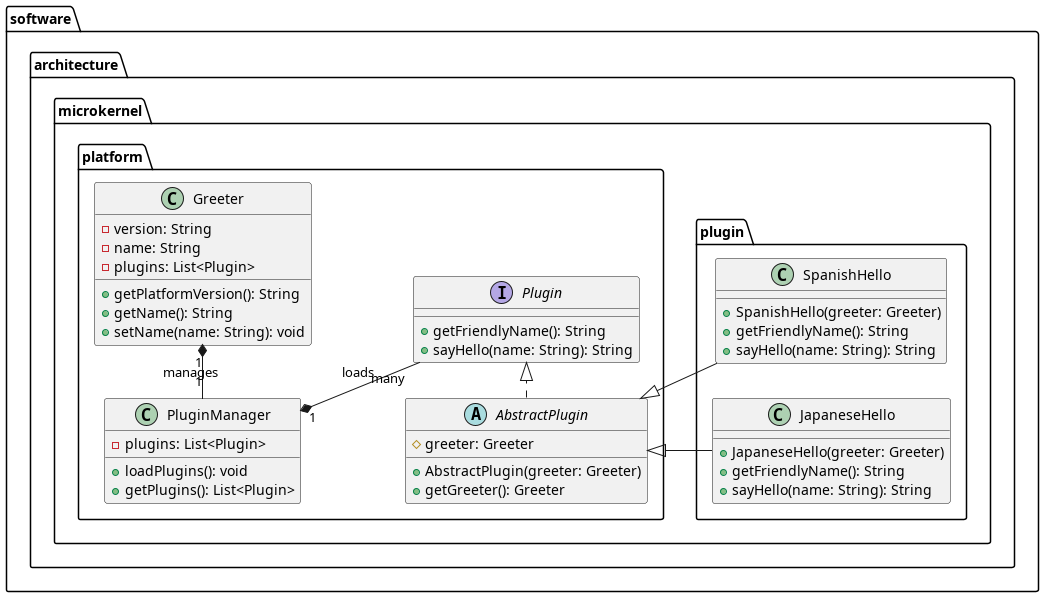
\includegraphics[width=\textwidth]{../images/out/plugin_architecture}
	\caption{Plugin Architecture}
	\label{fig:plugin_architecture}
\end{figure}

\subsection{Antarmuka \texttt{Plugin}}

Antarmuka \texttt{Plugin} dalam arsitektur microkernel pada kasus ini berfungsi sebagai kontrak bagi semua plugin yang akan digunakan dalam sistem. Dengan menggunakan antarmuka ini, sistem dapat berinteraksi dengan berbagai implementasi plugin tanpa bergantung pada detail spesifik dari setiap kelas plugin.

\begin{lstlisting}[style=JavaStyle, caption={Antarmuka \texttt{Plugin}}, label={lst:plugin-interface}]
	package software.architecture.microkernel.platform;
	
	public interface Plugin {
		String getFriendlyName();
		String sayHello(String name);
	}
\end{lstlisting}

\noindent
Antarmuka ini mendefinisikan dua metode utama:

\begin{itemize}
	\item \textbf{\texttt{getFriendlyName()}}: Metode ini mengembalikan nama ramah dari plugin, yang dapat digunakan untuk menampilkan informasi mengenai plugin kepada pengguna.
	\item \textbf{\texttt{sayHello(String name)}}: Metode ini menerima sebuah string \texttt{name} dan mengembalikan salam yang telah dikustomisasi berdasarkan implementasi dari plugin.
\end{itemize}

Dengan mendeklarasikan antarmuka ini, setiap plugin yang dikembangkan dalam sistem harus mengimplementasikan metode-metode tersebut, memastikan bahwa semua plugin memiliki fungsionalitas yang konsisten. Ini memungkinkan arsitektur microkernel untuk secara dinamis memuat dan menggunakan plugin yang berbeda tanpa perlu mengetahui detail internalnya.

Penggunaan antarmuka ini mendukung prinsip \textbf{Open/Closed Principle (OCP)} dalam desain perangkat lunak, di mana sistem dapat diperluas dengan menambahkan plugin baru tanpa harus mengubah kode inti dari microkernel.


\subsection{Kelas Abstrak \texttt{AbstractPlugin}}

Kelas abstrak \texttt{AbstractPlugin} merupakan implementasi dasar dari antarmuka \texttt{Plugin}. Kelas ini bertindak sebagai kelas induk bagi semua plugin yang akan digunakan dalam sistem, menyediakan struktur dasar yang diperlukan untuk berinteraksi dengan \texttt{Greeter}.

\begin{lstlisting}[style=JavaStyle, caption={Kelas Abstrak \texttt{AbstractPlugin}}, label={lst:abstract-plugin}]
	package software.architecture.microkernel.platform;
	
	public abstract class AbstractPlugin implements Plugin {
		protected Greeter greeter;
		
		public AbstractPlugin(Greeter greeter) {
			this.greeter = greeter;
		}
	}
\end{lstlisting}

\noindent
Kelas ini memiliki beberapa elemen penting:

\begin{itemize}
	\item \textbf{\texttt{implements Plugin}}: Kelas ini mengimplementasikan antarmuka \texttt{Plugin}, sehingga setiap kelas turunan wajib menyediakan implementasi metode yang didefinisikan dalam \texttt{Plugin}.
	\item \textbf{\texttt{protected Greeter greeter}}: Variabel ini memungkinkan setiap plugin untuk mengakses instance dari \texttt{Greeter}, yang berfungsi sebagai pengelola utama dalam sistem.
	\item \textbf{\texttt{public AbstractPlugin(Greeter greeter)}}: Konstruktor ini menginisialisasi objek \texttt{greeter}, memastikan bahwa setiap plugin yang dibuat memiliki referensi ke \texttt{Greeter}.
\end{itemize}

Dengan menggunakan kelas abstrak ini, pengembang dapat dengan mudah membuat plugin baru dengan hanya mengimplementasikan metode yang didefinisikan dalam \texttt{Plugin}, tanpa harus menangani detail implementasi dasar yang sudah disediakan oleh \texttt{AbstractPlugin}. Hal ini membantu menjaga prinsip **kode yang dapat digunakan kembali** dan memudahkan perluasan sistem microkernel.


\subsection{Kelas \texttt{SpanishHello}}

Kelas \texttt{SpanishHello} merupakan salah satu implementasi plugin dari sistem microkernel yang bertanggung jawab untuk memberikan salam dalam bahasa Spanyol. Kelas ini mewarisi \texttt{AbstractPlugin}, sehingga memperoleh akses ke objek \texttt{Greeter} yang digunakan dalam platform.

\begin{lstlisting}[style=JavaStyle, caption={Kelas \texttt{SpanishHello}}, label={lst:spanish-hello}]
	package software.architecture.microkernel.plugin;
	
	import software.architecture.microkernel.platform.Greeter;
	import software.architecture.microkernel.platform.AbstractPlugin;
	
	public class SpanishHello extends AbstractPlugin {
		
		public SpanishHello(Greeter greeter) {
			super(greeter);
			System.out.println(getFriendlyName() + " is loaded by Greeter " 
			+ greeter.getPlatformVersion());
		}
		
		@Override
		public String getFriendlyName() {
			return "Greet in Spanish";
		}
		
		@Override
		public String sayHello(String name) {
			return "Hola, " + name + "!";
		}
	}
\end{lstlisting}

\noindent
Kelas ini memiliki beberapa elemen utama:

\begin{itemize}
	\item \textbf{\texttt{extends AbstractPlugin}}: Kelas ini merupakan subclass dari \texttt{AbstractPlugin}, sehingga mendapatkan fungsionalitas dasar dari kelas induk.
	\item \textbf{\texttt{public SpanishHello(Greeter greeter)}}: Konstruktor yang menerima instance dari \texttt{Greeter} sebagai argumen dan meneruskannya ke konstruktor \texttt{AbstractPlugin}. Konstruktor ini juga mencetak pesan bahwa plugin telah berhasil dimuat.
	\item \textbf{\texttt{public String getFriendlyName()}}: Metode ini mengembalikan nama tampilan dari plugin, yaitu \texttt{"Greet in Spanish"}.
	\item \textbf{\texttt{public String sayHello(String name)}}: Metode ini menghasilkan salam dalam bahasa Spanyol dengan format \texttt{"Hola, <name>!"}.
\end{itemize}

Kelas \texttt{SpanishHello} menunjukkan bagaimana sebuah plugin dapat diintegrasikan ke dalam sistem microkernel. Dengan hanya mengimplementasikan metode dari antarmuka \texttt{Plugin}, kelas ini dapat ditambahkan ke dalam sistem tanpa perlu memodifikasi inti dari platform.

\subsection{Kelas \texttt{JapaneseHello}}

Kelas \texttt{JapaneseHello} adalah salah satu implementasi plugin dalam sistem microkernel yang bertanggung jawab untuk memberikan salam dalam bahasa Jepang. Kelas ini mewarisi \texttt{AbstractPlugin}, yang berarti mendapatkan akses ke objek \texttt{Greeter} dari platform.

\begin{lstlisting}[style=JavaStyle, caption={Kelas \texttt{JapaneseHello}}, label={lst:japanese-hello}, inputencoding=utf8]
	package software.architecture.microkernel.plugin;
	
	import software.architecture.microkernel.platform.Greeter;
	import software.architecture.microkernel.platform.AbstractPlugin;
	
	public class JapaneseHello extends AbstractPlugin {
		
		public JapaneseHello(Greeter greeter) {
			super(greeter);
			System.out.println(getFriendlyName() + " is loaded by Greeter " 
			+ greeter.getPlatformVersion());
		}
		
		@Override
		public String getFriendlyName() {
			return "Greet in Japanese";
		}
		
		@Override
		public String sayHello(String name) {
			return "XXXXX, " + name + "!";
		}
	}
\end{lstlisting}




\noindent
Kelas ini memiliki beberapa elemen utama:

\begin{itemize}
	\item \textbf{\texttt{extends AbstractPlugin}}: Kelas ini merupakan subclass dari \texttt{AbstractPlugin}, sehingga mendapatkan fungsionalitas dasar yang sama dengan plugin lainnya.
	\item \textbf{\texttt{public JapaneseHello(Greeter greeter)}}: Konstruktor menerima instance dari \texttt{Greeter} sebagai argumen dan meneruskannya ke konstruktor \texttt{AbstractPlugin}. Selain itu, mencetak pesan bahwa plugin telah berhasil dimuat.
	\item \textbf{\texttt{public String getFriendlyName()}}: Metode ini mengembalikan nama tampilan dari plugin, yaitu \texttt{"Greet in Japanese"}.
	\item \textbf{\texttt{public String sayHello(String name)}}: Metode ini menghasilkan salam dalam bahasa Jepang dengan format \texttt{"XXXXX, <name>!"}.
\end{itemize}

Dengan desain ini, \texttt{JapaneseHello} dapat dimuat secara dinamis oleh sistem microkernel tanpa perlu memodifikasi inti dari platform. Arsitektur ini memungkinkan fleksibilitas tinggi dalam menambahkan dan mengelola plugin.

\subsection{Kelas \texttt{PluginManager}}

Kelas \texttt{PluginManager} bertanggung jawab untuk mengelola siklus hidup plugin dalam arsitektur \textbf{Microkernel}. Kelas ini memungkinkan pemuatan plugin secara dinamis dari direktori eksternal dan memastikan bahwa plugin yang dimuat sesuai dengan antarmuka \texttt{Plugin}. 

\begin{lstlisting}[style=JavaStyle, caption={Kelas \texttt{PluginManager}}, label={lst:plugin-manager}, inputencoding=utf8]
	package software.architecture.microkernel.platform;
	
	import java.io.File;
	import java.io.InputStream;
	import java.lang.reflect.Constructor;
	import java.net.URL;
	import java.net.URLClassLoader;
	import java.util.*;
	
	public class PluginManager {
		
		private final Greeter greeter;
		private final List<Plugin> plugins = new ArrayList<>();
		
		public PluginManager(Greeter greeter) {
			this.greeter = greeter;
		}
		
		public void loadPlugins() {
			try {
				File pluginDir = new File("plugins");
				if (!pluginDir.exists() || !pluginDir.isDirectory()) {
					System.out.println("No plugins directory found.");
					return;
				}
				
				File[] jarFiles = pluginDir.listFiles((dir, name) -> name.endsWith(".jar"));
				if (jarFiles == null || jarFiles.length == 0) {
					System.out.println("No plugins found.");
					return;
				}
				
				for (File jar : jarFiles) {
					URLClassLoader classLoader = new URLClassLoader(new URL[]{jar.toURI().toURL()}, getClass().getClassLoader());
					InputStream propertiesInputStream = classLoader.getResourceAsStream("plugin.properties");
					
					if (propertiesInputStream == null) {
						System.out.println("Missing plugin.properties in " + jar.getName());
						continue;
					}
					
					Properties properties = new Properties();
					properties.load(propertiesInputStream);
					String mainClassName = properties.getProperty("mainclass");
					
					if (mainClassName == null || mainClassName.isEmpty()) {
						System.out.println("Invalid mainclass entry in " + jar.getName());
						continue;
					}
					
					Class<?> classToLoad = Class.forName(mainClassName, true, classLoader);
					Class<? extends Plugin> pluginClass = classToLoad.asSubclass(Plugin.class);
					Constructor<? extends Plugin> constructor = pluginClass.getDeclaredConstructor(Greeter.class);
					Plugin plugin = constructor.newInstance(greeter);
					plugins.add(plugin);
				}
				
			} catch (Exception e) {
				e.printStackTrace();
			}
		}
		
		public List<Plugin> getPlugins() {
			return plugins;
		}
	}
\end{lstlisting}

Kelas ini memiliki beberapa tanggung jawab utama:

\begin{itemize}
	\item \textbf{Memuat plugin dari direktori \texttt{plugins}/} \\
	Fungsi \texttt{loadPlugins()} mencari file \texttt{.jar} dalam direktori \texttt{plugins} dan menggunakan \texttt{URLClassLoader} untuk memuat kelas utama dari plugin.
	
	\item \textbf{Membaca konfigurasi plugin dari \texttt{plugin.properties}} \\
	Setiap plugin harus memiliki file \texttt{plugin.properties} yang menentukan kelas utama plugin dalam entri \texttt{mainclass}. Jika file atau entri ini tidak ditemukan, plugin tidak akan dimuat.
	
	\item \textbf{Menggunakan refleksi untuk menginisialisasi plugin} \\
	Setelah menemukan kelas utama plugin, kelas \texttt{PluginManager} menggunakan mekanisme refleksi untuk membuat instance dari plugin, dengan menyertakan referensi ke objek \texttt{Greeter}.
	
	\item \textbf{Menyimpan daftar plugin yang dimuat} \\
	Semua plugin yang berhasil dimuat akan disimpan dalam daftar \texttt{plugins}, yang dapat diakses melalui metode \texttt{getPlugins()}.
\end{itemize}

Kelas \texttt{PluginManager} adalah komponen kunci dalam arsitektur Microkernel, memungkinkan ekstensi fungsionalitas tanpa harus mengubah kode utama sistem.

\section{Kompilasi dan Menjalankan Aplikasi}

Aplikasi berbasis \textbf{Microkernel} ini menggunakan \textbf{Maven} sebagai alat bantu untuk membangun (\textit{build}) dan mengelola dependensi. Proses kompilasi dan eksekusi dilakukan dalam dua tahap utama:

\begin{enumerate}
	\item Membangun (\textit{package}) proyek platform utama (\texttt{Greeter}).
	\item Membangun setiap plugin sebagai proyek Maven yang terpisah.
	\item Memindahkan berkas \texttt{.jar} hasil kompilasi plugin ke dalam folder \texttt{plugins} pada proyek platform.
	\item Menjalankan aplikasi platform, yang secara otomatis memuat semua plugin yang tersedia.
\end{enumerate}

\subsection{Membangun dan Menginstal Proyek Platform}

Untuk membangun proyek utama yang berisi \texttt{Greeter}, jalankan perintah berikut di dalam direktori proyek \textbf{platform}:

\begin{lstlisting}[language=bash, caption={Membangun Proyek Platform Menggunakan Maven}]
	mvn clean package install
\end{lstlisting}

Setelah perintah ini dijalankan, Maven akan:

\begin{itemize}
	\item Mengunduh dan mengelola semua dependensi yang diperlukan.
	\item Mengkompilasi kode sumber platform.
	\item Menghasilkan berkas \texttt{.jar} di dalam direktori \texttt{target/}.
\end{itemize}

\subsection{Membangun Plugin}

Setiap plugin, seperti \texttt{JapaneseHello} dan \texttt{SpanishHello}, harus dikompilasi dan dikemas sebagai \texttt{.jar} secara terpisah. Untuk membangun setiap plugin, navigasikan ke direktori masing-masing plugin dan jalankan:

\begin{lstlisting}[language=bash, caption={Membangun Plugin Menggunakan Maven}]
	mvn clean package 
\end{lstlisting}

Hasil kompilasi akan berada di dalam direktori \texttt{target/} dengan nama sesuai konfigurasi \texttt{pom.xml}.

\subsection{Memindahkan Plugin ke Direktori \texttt{plugins}}

Setelah semua plugin berhasil dikompilasi dan dikemas sebagai \texttt{.jar}, langkah berikutnya adalah memindahkan berkas-berkas tersebut ke dalam folder \texttt{plugins} yang ada di dalam proyek \textbf{platform}. Gunakan perintah berikut untuk memindahkan hasil kompilasi:

\begin{lstlisting}[language=bash, caption={Memindahkan Plugin ke Direktori \texttt{plugins}}]
	mv target/*.jar ../platform/plugins/
\end{lstlisting}

\subsection{Menjalankan Aplikasi Platform}

Setelah semua plugin berada dalam direktori \texttt{plugins}, aplikasi \texttt{Greeter} dapat dijalankan. Sistem akan secara otomatis memuat semua plugin yang tersedia dan menampilkannya dalam daftar pilihan bahasa. Jalankan aplikasi menggunakan perintah:

\begin{lstlisting}[language=bash, caption={Menjalankan Aplikasi Platform}]
	mvn run 
	# atau
	java -jar target/platform.jar
\end{lstlisting}

\subsection{Output Program}

Jika semua langkah telah dilakukan dengan benar, aplikasi akan menampilkan output berikut:

\begin{lstlisting}[language=bash, caption={Contoh Output Saat Menjalankan Aplikasi}]
	Greet in Japanese is loaded by Greeter v1.0.1
	Greet in Spanish is loaded by Greeter v1.0.1
	Select the language to greet in:
	1. Greet in Japanese
	2. Greet in Spanish
	0. Quit
	Input: 1
	
	XXXXX, Alice!
	
	Select the language to greet in:
	1. Greet in Japanese
	2. Greet in Spanish
	0. Quit
	Input: 2
	
	Hola, Alice!
	
	Select the language to greet in:
	1. Greet in Japanese
	2. Greet in Spanish
	0. Quit
	Input:
\end{lstlisting}

Dengan pendekatan ini, sistem dapat memuat plugin secara dinamis tanpa perlu melakukan perubahan atau kompilasi ulang pada kode sumber utama. Setiap plugin cukup dikompilasi secara terpisah dan ditambahkan ke direktori \texttt{plugins}, menjadikan arsitektur ini fleksibel dan modular.


\section{Kesimpulan}

Arsitektur \textbf{microkernel} dan \textbf{plugin} merupakan dua pendekatan yang digunakan untuk meningkatkan modularitas, fleksibilitas, dan skalabilitas dalam pengembangan perangkat lunak. Microkernel memungkinkan pemisahan layanan sistem dari kernel utama, sehingga meningkatkan keamanan dan ketahanan terhadap kegagalan. Sementara itu, plugin architecture memberikan fleksibilitas dengan memungkinkan ekstensi fungsionalitas tanpa mengubah kode inti sistem.

Meskipun microkernel menawarkan keunggulan dalam stabilitas dan keamanan, pendekatan ini memiliki tantangan dalam hal efisiensi komunikasi antar-proses dan kompleksitas implementasi. Oleh karena itu, penerapan microkernel lebih umum digunakan dalam sistem yang membutuhkan keandalan tinggi seperti sistem tertanam, sistem operasi real-time, dan hypervisor virtualisasi.

Di sisi lain, plugin architecture banyak digunakan dalam aplikasi perangkat lunak yang membutuhkan kemampuan ekspansi, seperti Integrated Development Environment (IDE), sistem manajemen konten (CMS), dan mesin game. Dengan menggunakan pendekatan ini, pengembang dapat memperluas fungsionalitas perangkat lunak tanpa perlu mengubah kode sumber utama, sehingga meningkatkan skalabilitas dan kemudahan pemeliharaan.

Melalui implementasi berbasis Java, dokumen ini telah menunjukkan bagaimana microkernel dan plugin dapat diterapkan dalam praktik, termasuk teknik pemuatan dinamis plugin menggunakan refleksi dan manajemen dependensi dengan Maven. Pendekatan ini memungkinkan pengembangan sistem yang lebih modular, terstruktur, dan mudah diperluas.

Dengan pemahaman yang lebih mendalam mengenai arsitektur microkernel dan plugin, pengembang dapat memilih strategi yang paling sesuai dengan kebutuhan sistem yang sedang dibangun. Baik untuk pengembangan sistem operasi maupun aplikasi perangkat lunak modern, kedua arsitektur ini tetap menjadi solusi utama dalam menciptakan sistem yang lebih fleksibel dan tangguh terhadap perubahan.

